\documentclass{article}

\usepackage{graphicx}
\usepackage{tikz}
\usepackage{tikzsymbols}
\usetikzlibrary{calc,patterns,shapes.geometric}
\pagestyle{empty}
\usepackage[margin=0pt]{geometry}
\geometry{papersize={14in,12in}}

\def\centerarc[#1](#2)(#3:#4:#5){\draw[#1] ($(#2)+({#5*cos(#3)},{#5*sin(#3)})$) arc (#3:#4:#5);}

\begin{document}
	\begin{figure}
		\centering
		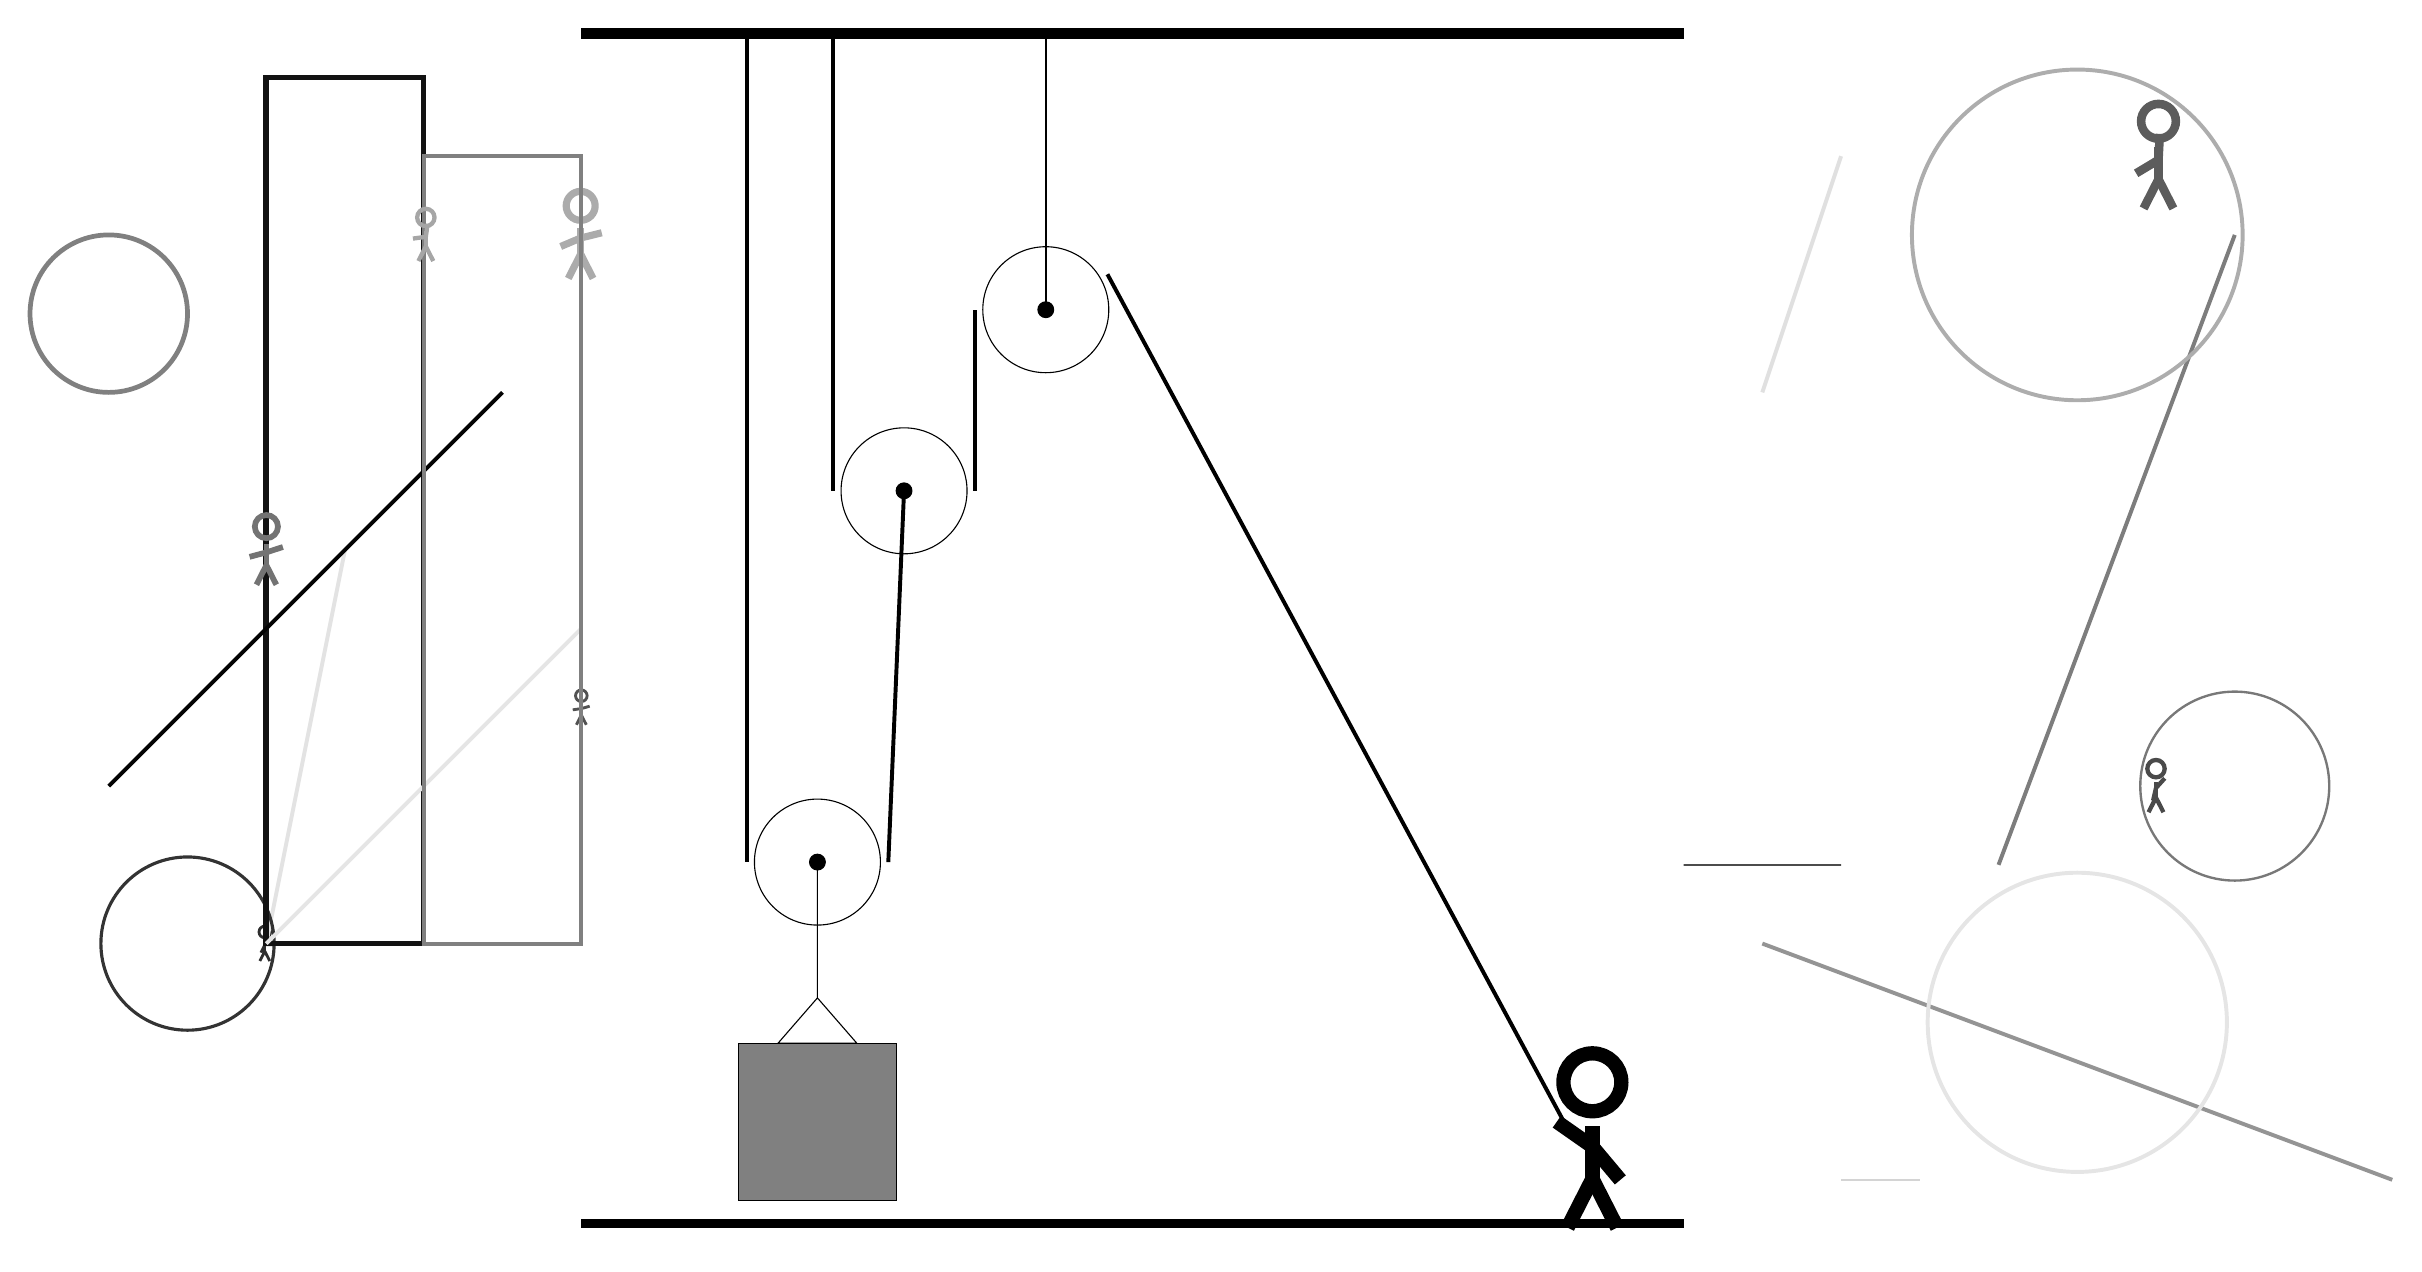
\begin{tikzpicture}
			%%%%% START %%%%%
			
			\draw[fill=black] (-2, 11.5) rectangle (12, 11.625);
			
			\draw [line width=0.3mm, color=black!53](19, 2) circle (1.2);
			
			\node[line width=0.5mm, color=black!64] at (18, 10) {\Strichmaxerl[6][31][87]};
			\draw[line width=0.5mm, color=black!42](13, 0) -- (21, -3);
			\draw[line width=0.5mm, color=black!12](14, 10) -- (13, 7);
			
			\draw[line width=0.5mm, color=black!28](16, -2) -- (16, -2);
			\node[line width=0.2mm, color=black!82] at (-6, 0) {\Strichmaxerl[2][64][1]};
			
			\draw [line width=0.6mm, color=black!50](-8, 8) circle (1.0);
			\draw[line width=0.3mm, color=black!17] (14, -3) rectangle (15, -3);
			\node[line width=0.4mm, color=black!71] at (18, 2) {\Strichmaxerl[3][77][48]};
			
			\draw[line width=0.5mm, color=black!11](-5, 5) -- (-6, 0);
			\draw [line width=0.5mm, color=black!10](17, -1) circle (1.9);
			\draw [line width=0.4mm, color=black!80](-7, 0) circle (1.1);
			\node[line width=0.2mm, color=black!68] at (-2, 3) {\Strichmaxerl[2][8][16]};
			
			\draw[line width=0.5mm, color=black!51](16, 1) -- (19, 9);
			\node[line width=0.5mm, color=black!33] at (-2, 9) {\Strichmaxerl[5][23][14]};
			\draw[line width=0.7mm, color=black!93] (-4, 11) rectangle (-6, 0);
			\draw[line width=0.5mm, color=black!10](-2, 4) -- (-6, 0);
			\node[line width=0.4mm, color=black!55] at (-6, 5) {\Strichmaxerl[4][15][18]};
			\draw[line width=0.2mm, color=black!70] (14, 1) rectangle (12, 1);
			\draw [line width=0.5mm, color=black!32](17, 9) circle (2.1);
			\draw[line width=0.5mm, color=black!99](-3, 7) -- (-8, 2);
			\draw[line width=0.5mm, color=black!50] (-4, 0) rectangle (-2, 10);
			\node[line width=0.7mm, color=black!35] at (-4, 9) {\Strichmaxerl[3][8][82]};
			
			\draw (1, 1.035) circle (0.8);
			\draw[fill=black] (1, 1.035) circle (0.1);
			
			\draw (2.1, 5.75) circle (0.8);
			\draw[fill=black] (2.1, 5.75) circle (0.1);
			
			\draw (3.9, 8.05) circle (0.8);
			\draw[fill=black] (3.9, 8.05) circle (0.1);
			\draw[thick] (3.9, 8.05) -- (3.9, 11.5);
			
			\draw (1, 1.035) -- (1, -0.69) -- (0.5, -1.265) -- (1.5, -1.265) -- (1, -0.69);
			\draw[fill=black!50] (0, -1.265) rectangle (2, -3.265);
			
			\draw[line width=0.5mm] (0.1, 11.5) -- (0.1, 1.035);
			\centerarc[line width=0.5mm](1, 1.035)(180:360:0.9);
			\draw[line width=0.5mm](1.9, 1.035) -- (2.1, 5.75);
			\draw[line width=0.5mm] (1.2, 11.5) -- (1.2, 5.75);
			\centerarc[line width=0.5mm](2.1, 5.75)(180:360:0.9);
			\draw[line width=0.5mm](3.0, 5.75) -- (3.0, 8.05);
			\centerarc[line width=0.5mm](3.9, 8.05)(30:180:0.9);
			\draw[line width=0.5mm] (4.683, 8.5) -- (10.5, -2.3);
			
			\node at (10.8, -2.5) {\Strichmaxerl[10][-35][-50]};
			
			\draw[fill=black] (-2, -3.5) rectangle (12, -3.6);
			
			%%%%% END %%%%%
		\end{tikzpicture}
	\end{figure}	
\end{document}